This section documents the results on the $\WW$ cross-section measurement. 
The selections are the same as in the $\WW$ preselection defined in 
Section~\ref{sec:selection}, except for the following two differences:

\begin{enumerate}
\item the trailing lepton threshold is 20 $\GeV$;
\item the $\met$ selections used are from the high mass Higgs strategy;
\item make use of the 0-jet bin only.
\end{enumerate}


\subsection{Background Estimations}

The background estimations use the same method as in the Higgs search 
documented in Section~\ref{sec:backgrounds}.

The Drell-Yan and top background estimations are tabulated in 
Tables~\ref{tab:dy_wwxsec} and~\ref{tab:top_wwsec}, respectively.

%%%%%%%%%%%%%%%%%%%%%%%%%%%%%
\begin{table}[!hbtp]
\begin{center}
\begin{tabular}{l|cccc}
\hline
Final State & $N(\ell\ell)_{\textrm{control}}^{\textrm{data}}$  & $N_{\textrm{control}}^{\textrm{ZV, sim.}}$ & $R_{out/in}$ & $N_{out}$ (data) \\ 
\hline
ee                          & 147   & $38.5 \pm 0.5 \pm 3.8$    & $0.16 \pm 0.02 \pm 0.06$    & $14.6 \pm 3.0 \pm 5.2$  \\
$\mu\mu$                    & 223   & $57.5 \pm 0.5 \pm 5.8$    & $0.19 \pm 0.03 \pm 0.03$    & $25.7 \pm 4.7 \pm 4.6$ \\
$e\mu$                      & 49    & -                         & -                           & -\\ 
\hline
$ee$ and $\mu\mu$ combined  & 132  & $96.0 \pm 0.7 \pm 9.6$     & $0.18 \pm 0.02 \pm 0.04$    & $40.2 \pm 5.7 \pm 9.8$ \\
\hline
\end{tabular}
\end{center}
\caption{ Predictions of the off-peak $Z/\gamma^*$ contribution 
for events passing all $WW$ selections. Both statistical and systematic uncertainties 
are displayed. For the $VZ$ contribution in the control region, we assign 10\% systematics due to the 
uncertainty in the cross-sections. }
\label{tab:dy_wwxsec}
\end{table}
%%%%%%%%%%%%%%%%%%%%%%%%%%%%%%

%%%%%%%%%%%%%%%%%%%%%%
\begin{figure}[!hbtp]
\centering
\subfigure[ee]{
\centering
\label{subfig:dyr_ee_0j}
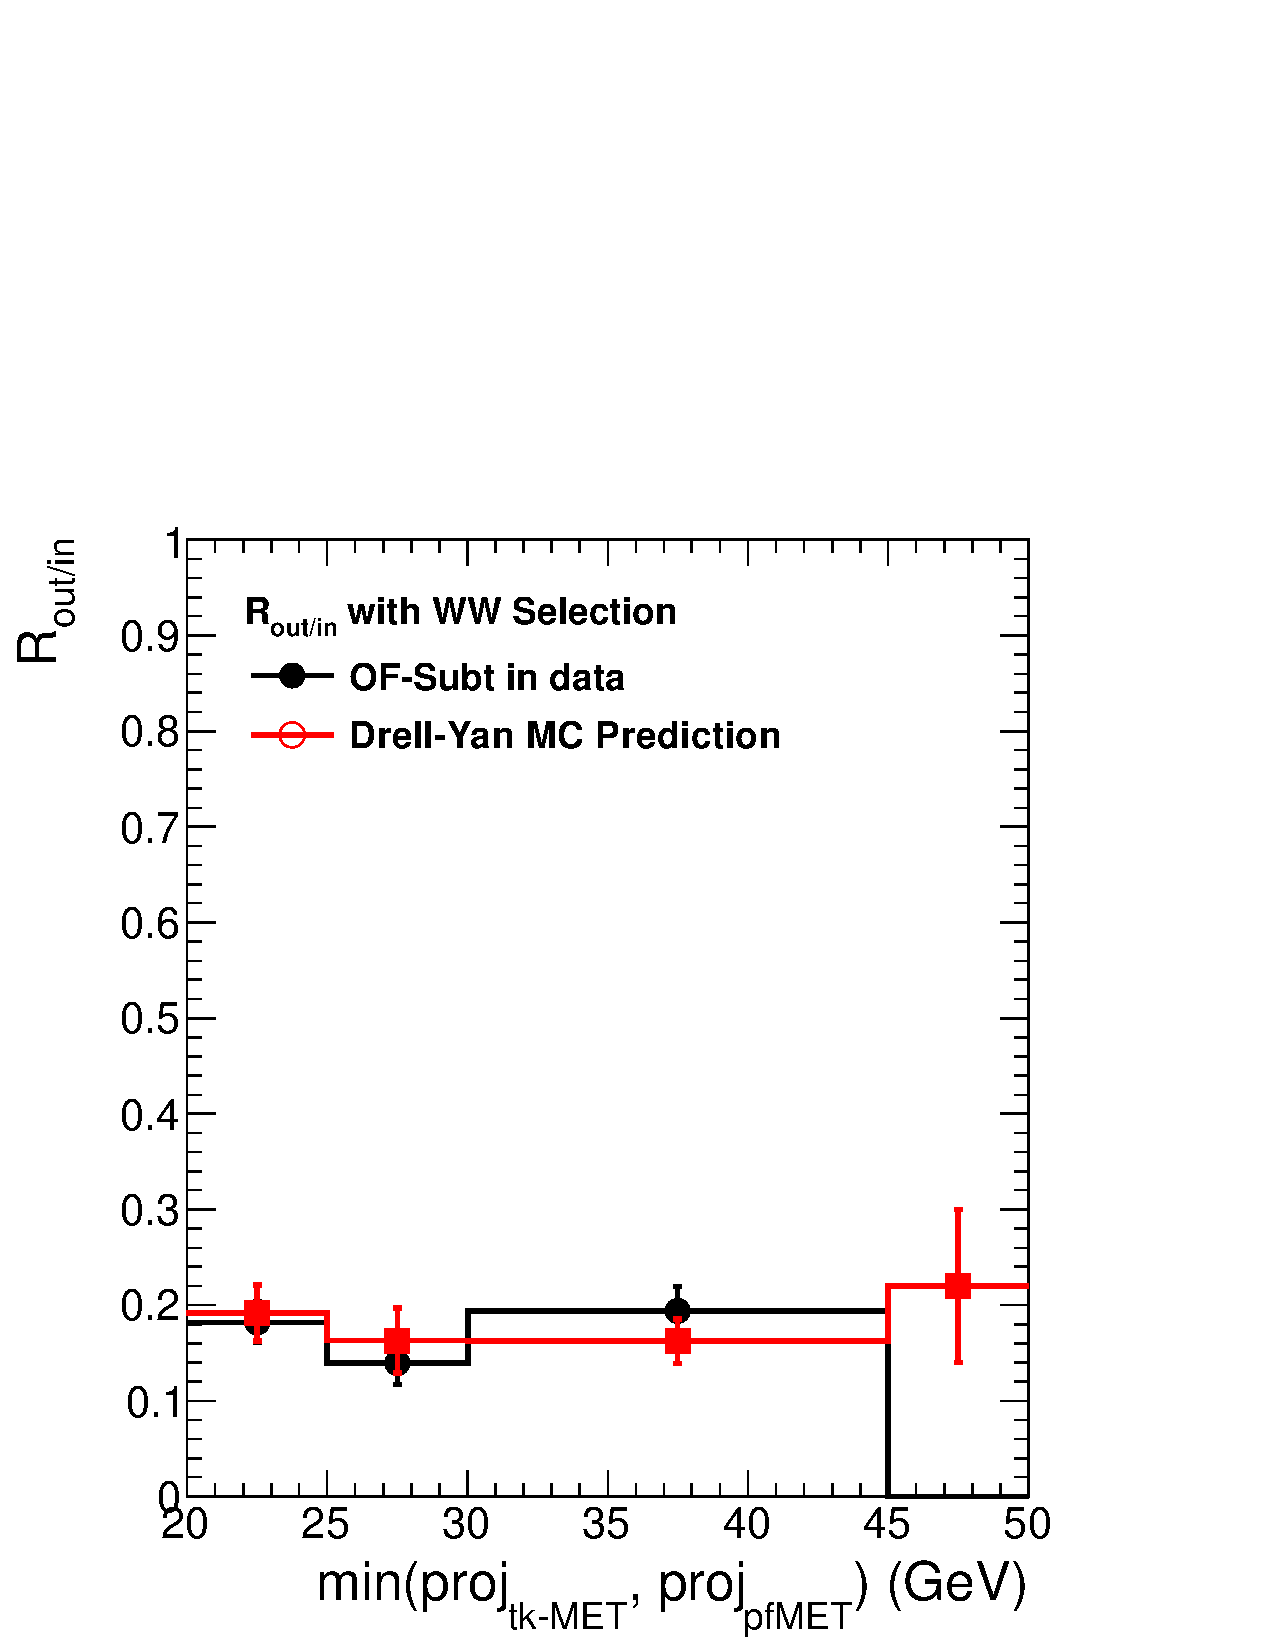
\includegraphics[width=.3\textwidth]{figures/Routin_ee_0Jet_mH0_3553pb_dy_wwxsec.pdf}}
\subfigure[mm]{
\centering
\label{subfig:dyr_mm_0j}
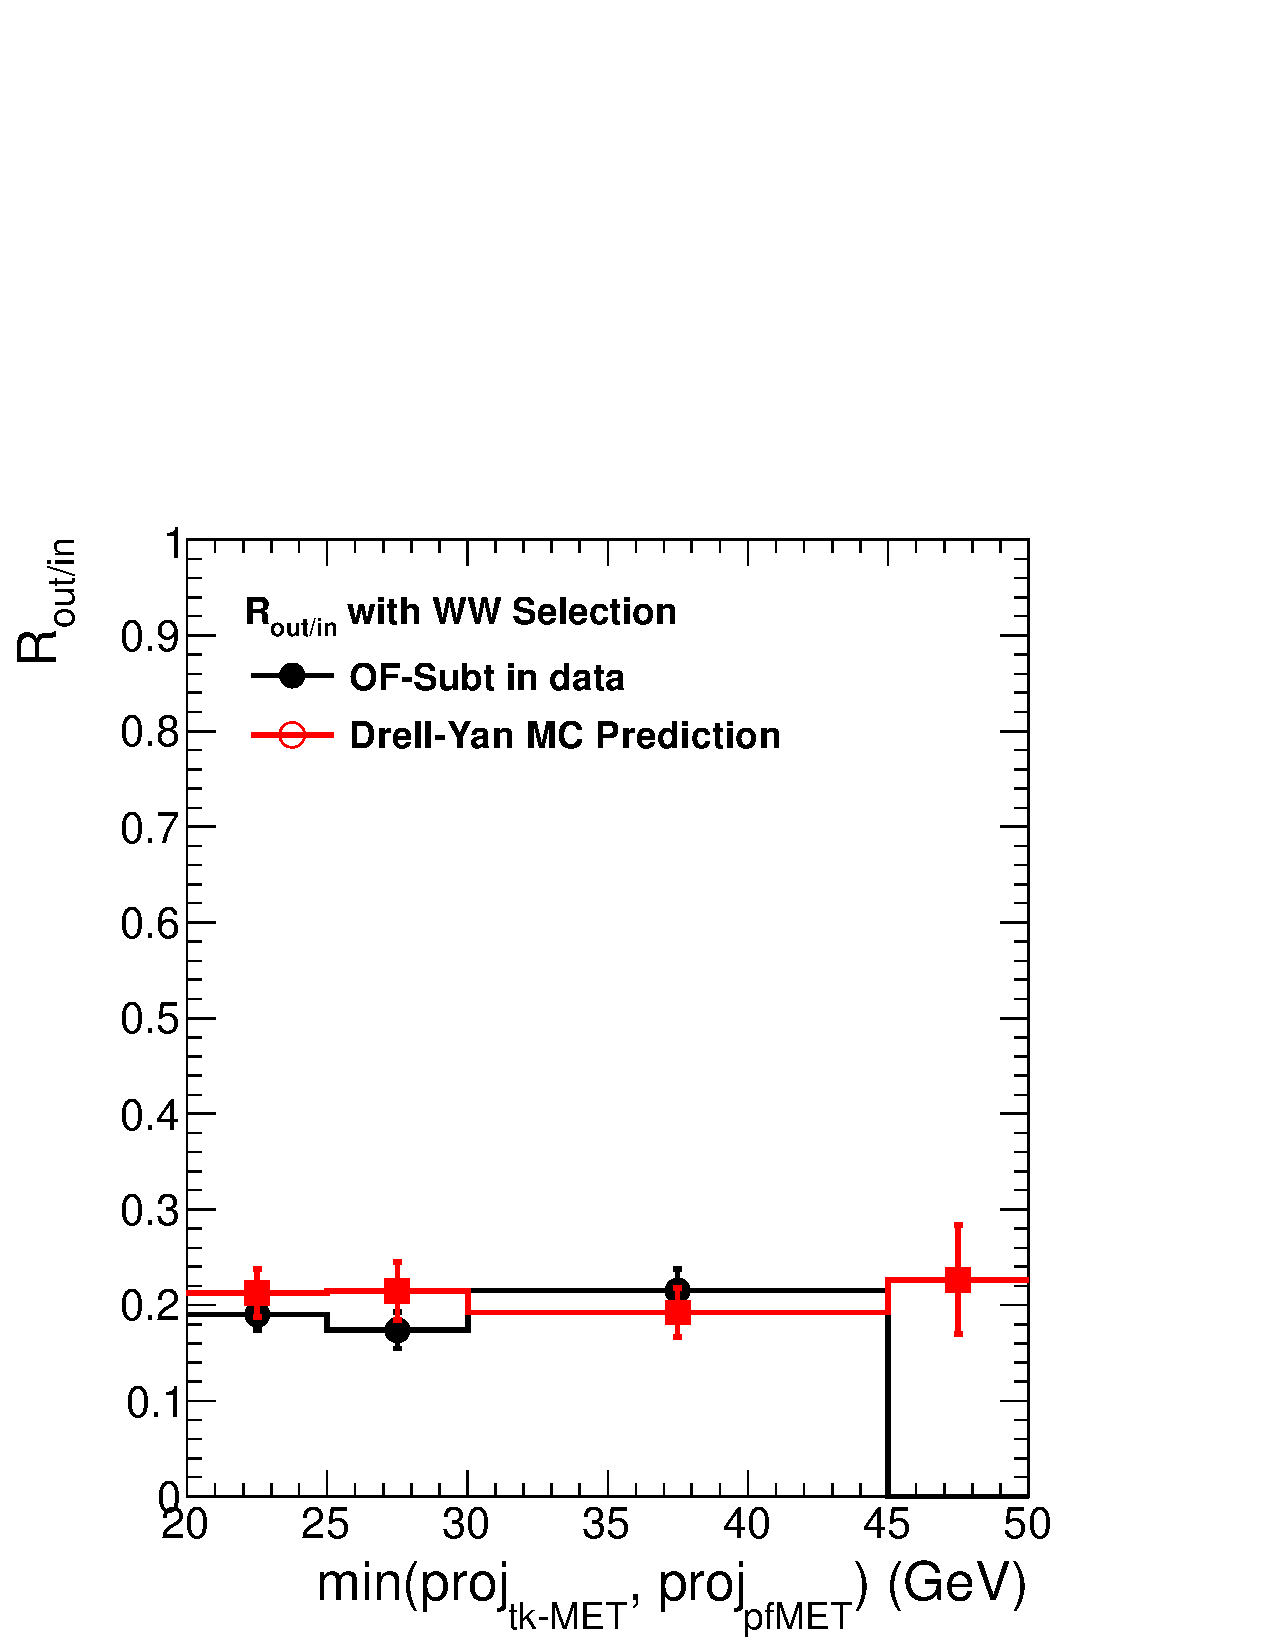
\includegraphics[width=.3\textwidth]{figures/Routin_mm_0Jet_mH0_3553pb_dy_wwxsec.pdf}}
\subfigure[ee/mm combined]{
\centering
\label{subfig:dyr_ll_0j}
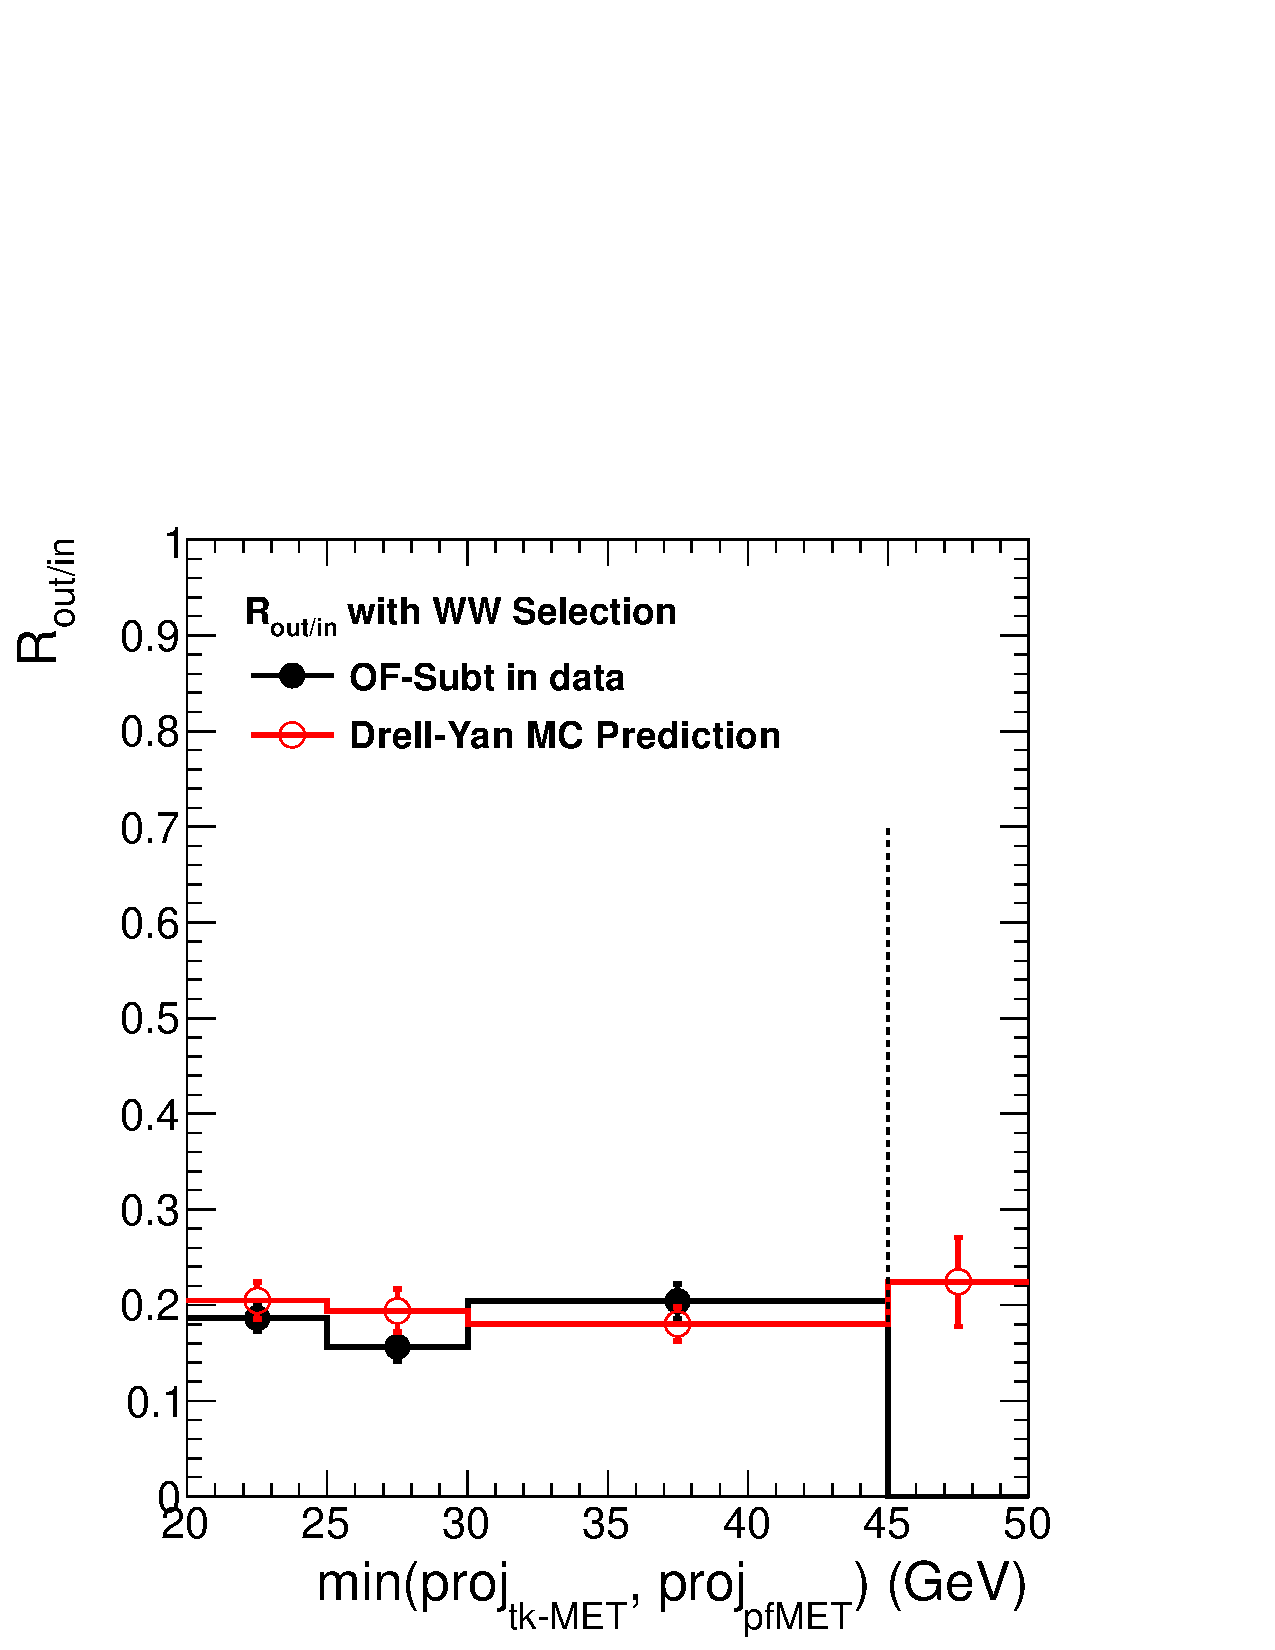
\includegraphics[width=.3\textwidth]{figures/Routin_0Jet_mH0_3553pb_dy_wwxsec.pdf}}
\caption{
 The \routin\, as a function of MET measured from data (black solid dots) 
and MC (red open circles) for the Drell-Yan processes. The measurements 
in data are done using the opposite flavor subtraction method, with the 
last bin blinded in data. }
\label{fig:dyr_ww}
\end{figure}
%%%%%%%%%%%%%%%%%%%%%%

%%%%%%%%%%%%%%%%%%%%%%%%%%%%%% 
\begin{table}[ht!]
\begin{center} 
\begin{tabular}{l c}
\hline
                             Parameter      & Value             \\
\hline
       Estimated top events in simulation   & 120.7  $\pm$ 6.5   \\
                   tagging efficiency (\%)  & 53.8 $\pm$  4.4   \\
                top-tagged events in data   & 192 \\ 
      background events in control region   & 39.5 $\pm$ 9.8  \\
      Data-driven top background estimate   & 130.9 $\pm$ 28.2  \\
                            Scale factors   & 1.08$\pm$ 0.23 \\
\hline
\end{tabular}  
\caption{Monte Carlo to data scale factor for the top background contribution for $\intlumiEightTeV$.}  
\label{tab:top_wwsec}
\end{center}
\end{table}
%%%%%%%%%%%%%%%%%%%%%%%%%%%%%%

\subsection{Systematic Uncertainties for the Cross-section Measurement}

The summary of all systematic uncertainties are shown in Table~\ref{tab:systww}.

\begin{table}[ht!]
\begin{center}
\caption{\label{tab:systww} Summary of all systematic uncertainties (relative).}
\vspace{5pt}
{\small
\begin{tabular}{l|c|c|c|c|c|c|c}%|c|c|c}
\hline
%\multirow{2}{*}{Source} & $qq \to$ & $gg \to$  & non-$\Z$ resonant & top & DY & $\Wjets$ & $V(W/Z)+\gamma$    \\
\multirow{2}{*}{Source} & $qq \to$ & $gg \to$  & $WZ$ & $ZZ$  & top & $Z/\gamma^*$         & $\Wjets$ \\ %& $W+\gamma$ &$W+\gamma*$&  $Z/\gamma^*$   \\
                        & $\WW$    & $\WW$     &      &       &     & $\rightarrow\ell\ell$&          \\ %&            &           &  $\rightarrow\tau\tau$  \\
\hline

\hline
Luminosity                    & 5.0 & 5.0 & 5.0 & 5.0 & --- & --- &  --- \\ %& --- & 5.0 & --- \\
Trigger efficiencies          & 1.5 & 1.5 & 1.5 & 1.5 & --- & --- &  --- \\ %& --- & 1.5 & ---\\
Muon efficiency               & 1.5 & 1.5 & 1.5 & 1.5 & --- & --- &  --- \\ %& --- & 1.5 & ---\\
Electron id efficiency        & 2.0 & 2.0 & 2.0 & 2.0 & --- & --- &  --- \\ %& --- & 2.0 & ---\\
Momentum scale                & 1.5 & 1.5 & 1.5 & 1.5 & --- & --- &  --- \\ %& --- & 1.5 & ---\\
$\met$ resolution             & 2.0 & 2.0 & 2.0 & 2.0 & --- & --- &  --- \\ %& --- & 2.0 & ---\\
Jet veto                      & 4.7 & 4.7 & 4.7 & 4.7 & --- & --- &  --- \\ %& --- & 4.7 & ---\\
PDF uncertainties             & 2.3 & 0.8 & 6.5 & 4.8 & --- & --- &  --- \\ %& --- & 4.8 & ---\\
QCD scale uncertainties       & 1.5 &  30 & 4.2 & 1.8 & --- & --- &  --- \\ %& --- & 1.8 & ---\\
Pile up                       & 2.0 & 2.0 & 2.0 & 2.0 & --- & --- &  --- \\ %& --- & 2.0 & --- \\
$\Wjets$ norm.                & --- & --- & --- & --- & --- & --- &  36  \\ %& --- & --- & ---\\
top  norm.                    & --- & --- & --- & --- & 25  & --- &  --- \\ %& --- & --- & ---\\
$\dyll$ norm.                 & --- & --- & --- & --- & --- &  40 &  --- \\ %& --- & --- & ---\\
%$\dytt$ norm.                 & --- & --- & --- & --- & --- &  ---&  --- & --- & --- & 10\\
%$\W+\gamma$ cross section     & --- & --- & --- & --- & --- & --- &  --- &  30 & --- & ---\\
%$\W+\gamma^{*}$ cross section & --- & --- & --- & --- & --- & --- &  --- & --- &  30 & ---\\
%\hline 
%Total systematic uncertainty  &  8  &   8 &  11 &  9  & 19  &  43  & 36  & 30 & --- & ---\\ 
\hline
\end{tabular}
}
\end{center}
\end{table}


\subsection{Cross-section Measurement}

We now calculate the $\WW$ production cross section according to equation \ref{eq:mainformula},

\begin{equation}
\label{eq:mainformula}
\sigma_{WW}  = \frac{N_{data} - N_{bkg}}{\epsilon \cdot {\cal{L}} \cdot BR(WW \to \ell \nu \ell \nu)}
\end{equation}

Where $N_{data}$ is the number of events observed in data, $N_{bkg}$ is the estimated number
of background events, which are summarised with their uncertainties in Table \ref{tab:data_yields}. 
The efficiency to select $\sigma_{WW \to 2\ell 2\nu}$
candidates, $\varepsilon$, is computed as the weighted mean of
the $qq\to\WW$ and $gg\to\WW$ efficiencies in simulation.
Assuming a 3\% contribution from the $gg$ process, 
$\varepsilon$ is found to be $(3.23 \pm 0.26)\%$.
The integrated luminosity of the data sample is ${\cal{L}} = $ $\intlumiEightTeV$ $\pm$ 5\%;
the branching ratio is $BR(W \to \ell \nu) =$ 0.1080 $\pm$ 0.0009~\cite{pdg} so that the total branching ratio
accounting for all leptoninc final states is $BR(W \to \ell \ell \nu \nu) =$ 9 $\cdot$ 0.1080 $\cdot$ 0.1080 = 0.1050 $\pm$ 0.0017.

\begin{table}[ht!]
  \begin{center}
  \begin{tabular} {|c|c|}
\hline
Sample & yield $\pm$ stat $\pm$ syst. \\ \hline
$qqWW$  & $645.07 \pm 4.92 \pm 46.33 $  \\
$qqWW$  & $43.54 \pm 0.96 \pm 13.38 $   \\ 
$t\bar{t} + tW$ & $130.89 \pm 7.04 \pm 28.27 $  \\
$W+jets$    & $56.27 \pm 5.11 \pm 20.26 $   \\$WZ$    & $20.09 \pm 0.36 \pm 2.27 $    \\$ZZ$    & $7.84 \pm 0.19 \pm 0.78 $ \\ 
$Z/\gamma*$ & $41.11 \pm 7.16 \pm 9.86 $    \\ 
$W\gamma*/W+\gamma$ & $20.70 \pm 3.35 \pm 6.21 $    \\
\hline \hline 
Total B.    & $276.90 \pm 11.76 \pm 36.76 $ \\ \hline \hline
Total B.+S. & $965.51 \pm 12.78 \pm 60.63 $ \\ \hline \hline
Data    & $1103$    \\ \hline \hline
Acceptance ( \% )   & $3.23 \pm 0.26    $\\ 
\hline

\end{tabular}
  \caption{Expected number of signal and background events from the data-driven methods for
  an integrated luminosity of $\intlumiEightTeV$ after applying the selection requirements 
in the $\mu\mu$, $\mu{e}$, $e\mu$ and $ee$  channels.
The $Z/\gamma*$ entry is the sum of the same flavor Drell-Yan background estimate,
the contribution of $Z+\mathrm{jets}$ in the different flavor channels,
and the $Z\rightarrow\tau\tau$ process.
}
   \label{tab:data_yields}
  \end{center}
\end{table}

Using the inputs described previously and Equation \ref{eq:mainformula},
we obtain the following $WW$ cross-section measurement:

\begin{equation*}
\wwCrossSectionMeasurement
\end{equation*}

%%%%%%%%
\begin{figure}[!hbtp]
\begin{center}
\subfigure[Leading lepton $p_{T}$]{\label{subfig:fig_inclplots_pt1}
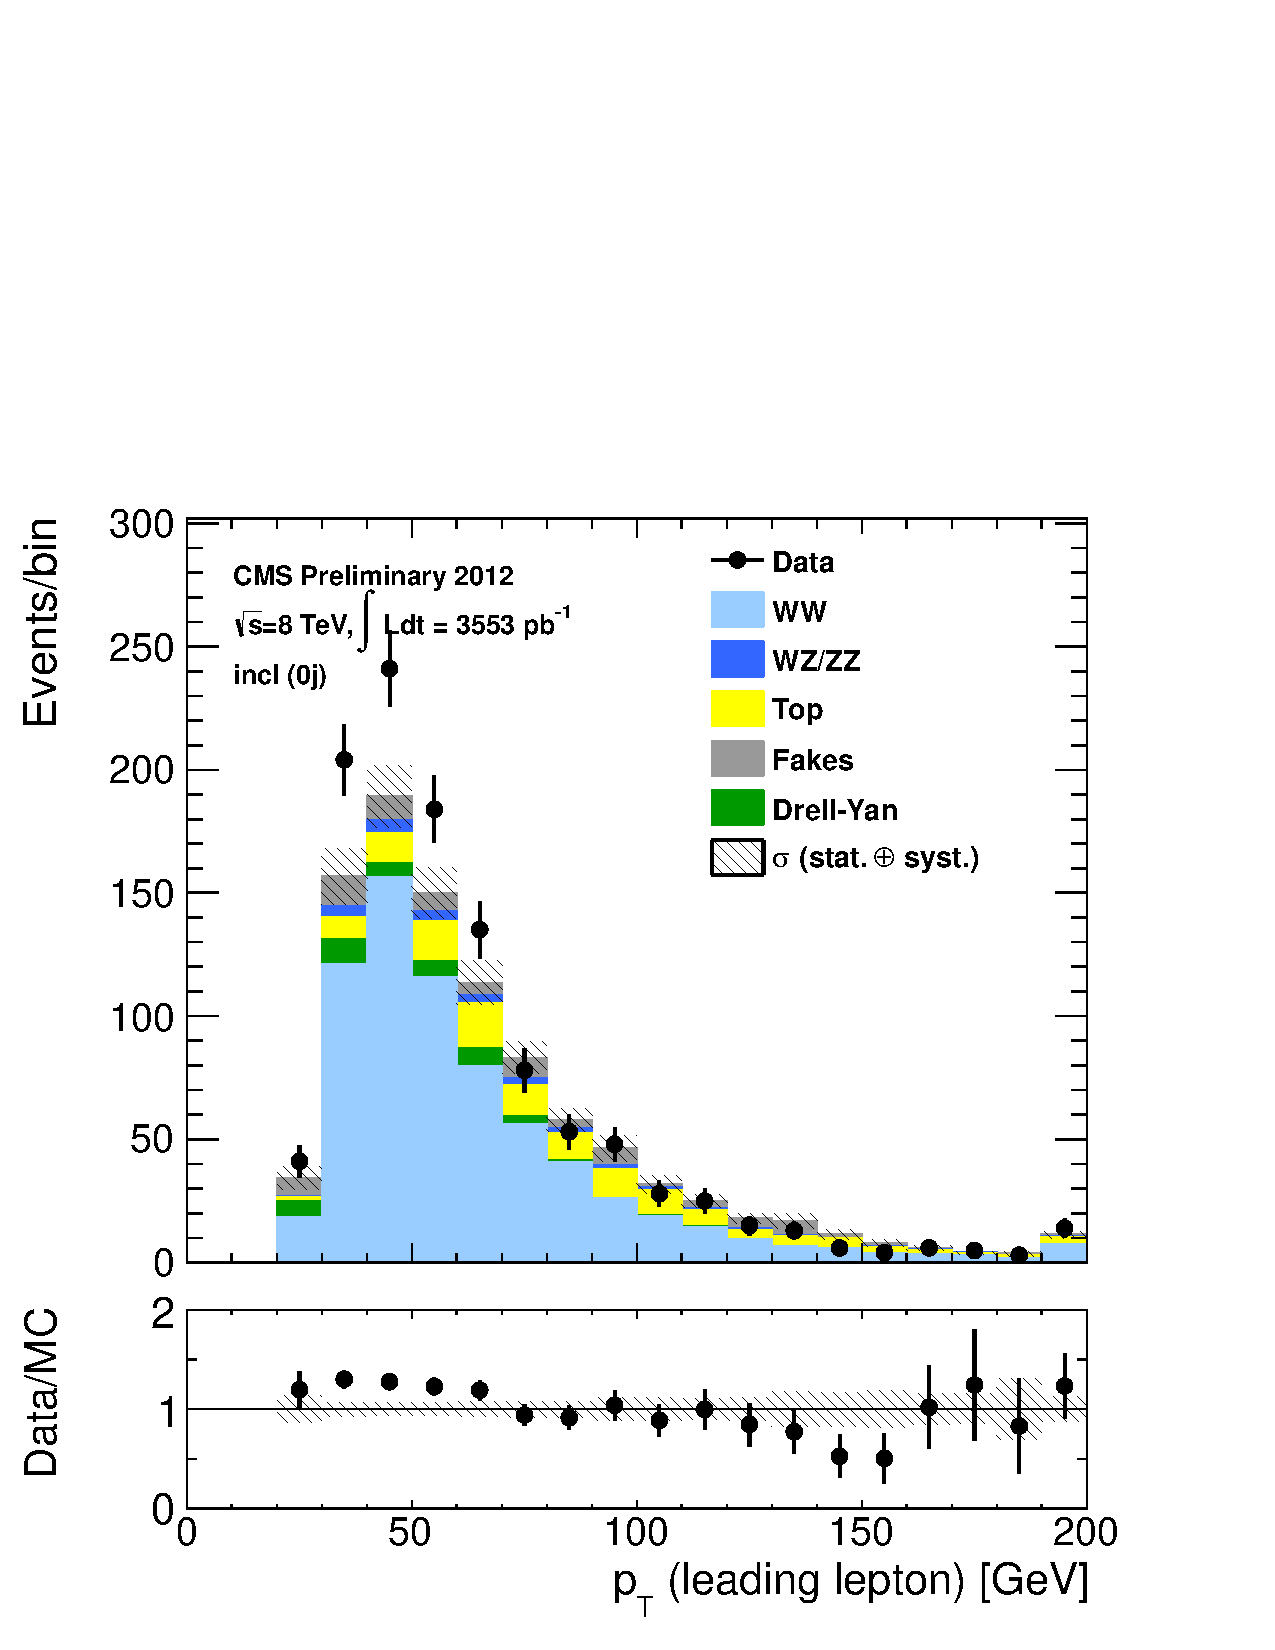
\includegraphics[width=.45\textwidth]{figures/ww_analysis20_pt1_incl_0j.pdf}}
\subfigure[Trailing lepton $p_{T}$]{\label{subfig:fig_inclplots_pt2}
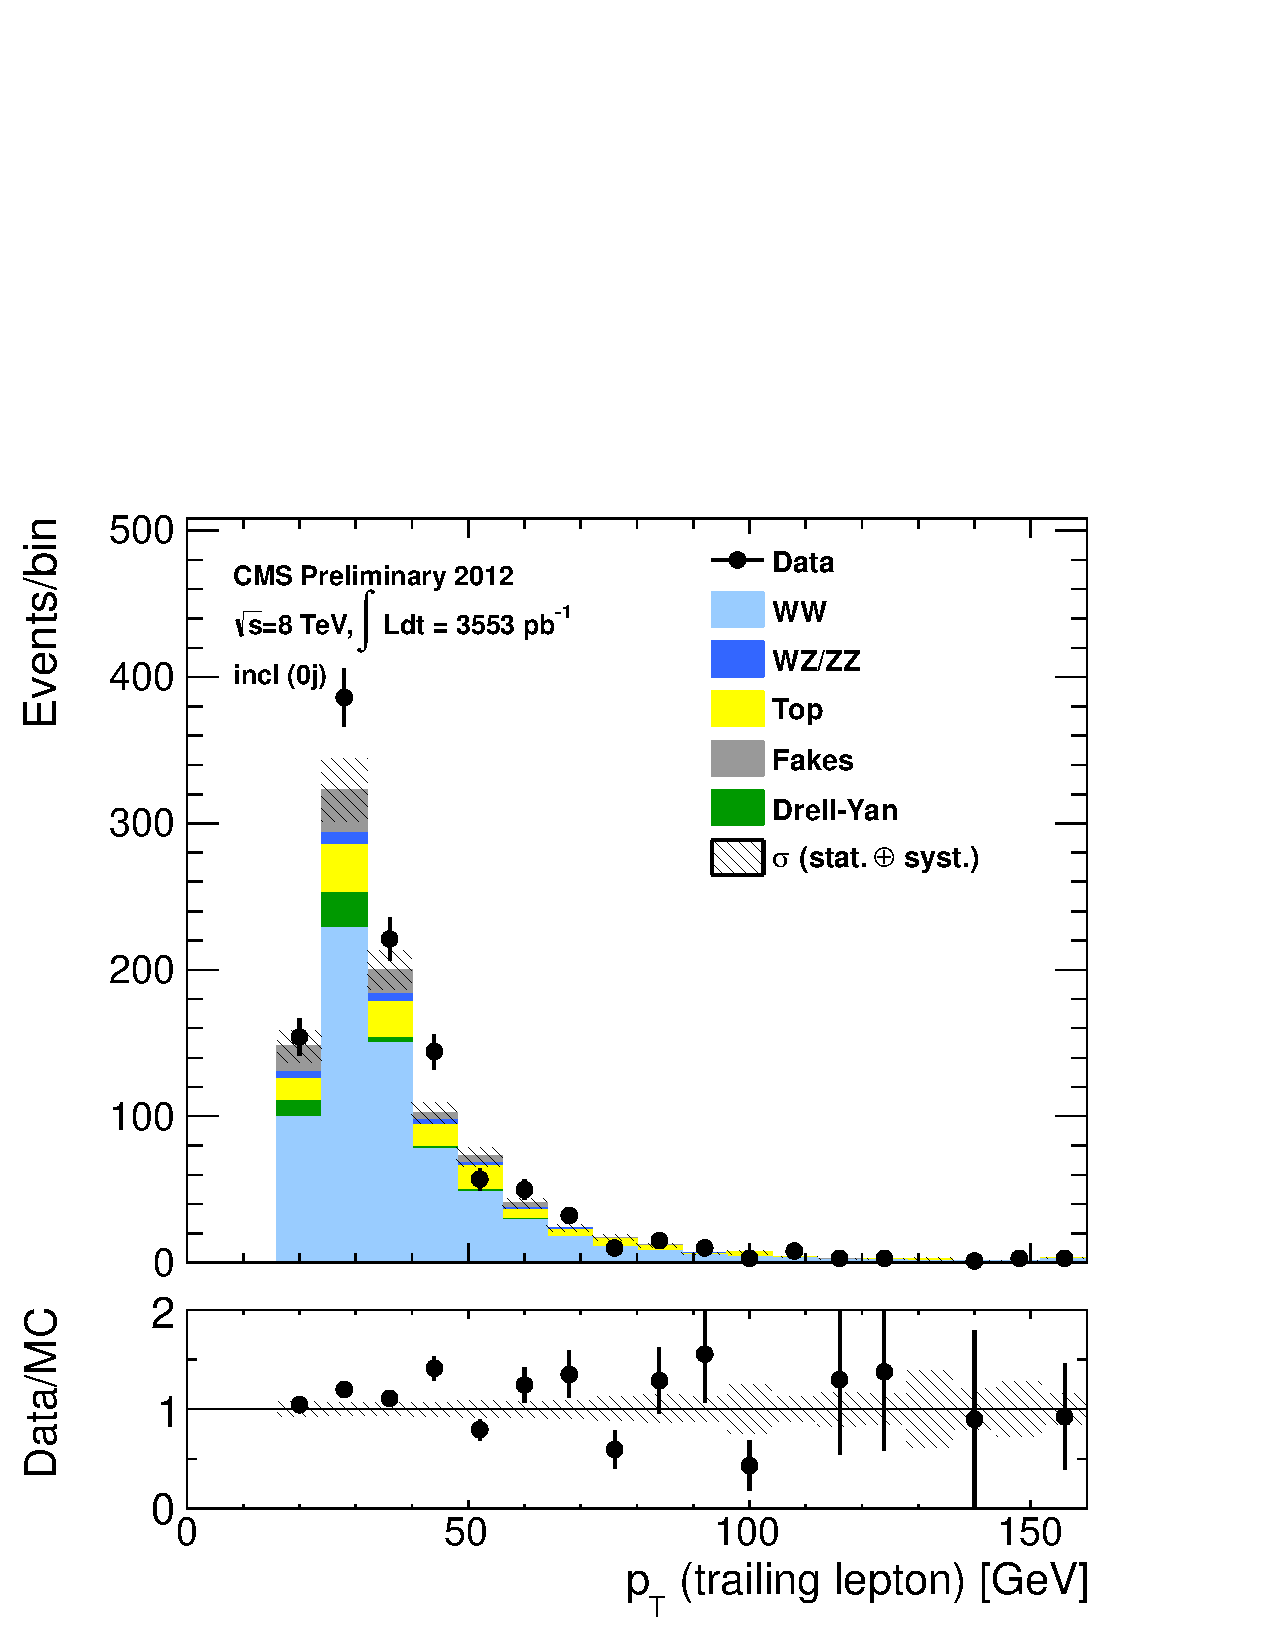
\includegraphics[width=.45\textwidth]{figures/ww_analysis20_pt2_incl_0j.pdf}}
\subfigure[Dilepton system $p_{T}$]{\label{subfig:fig_inclplots_ptll}
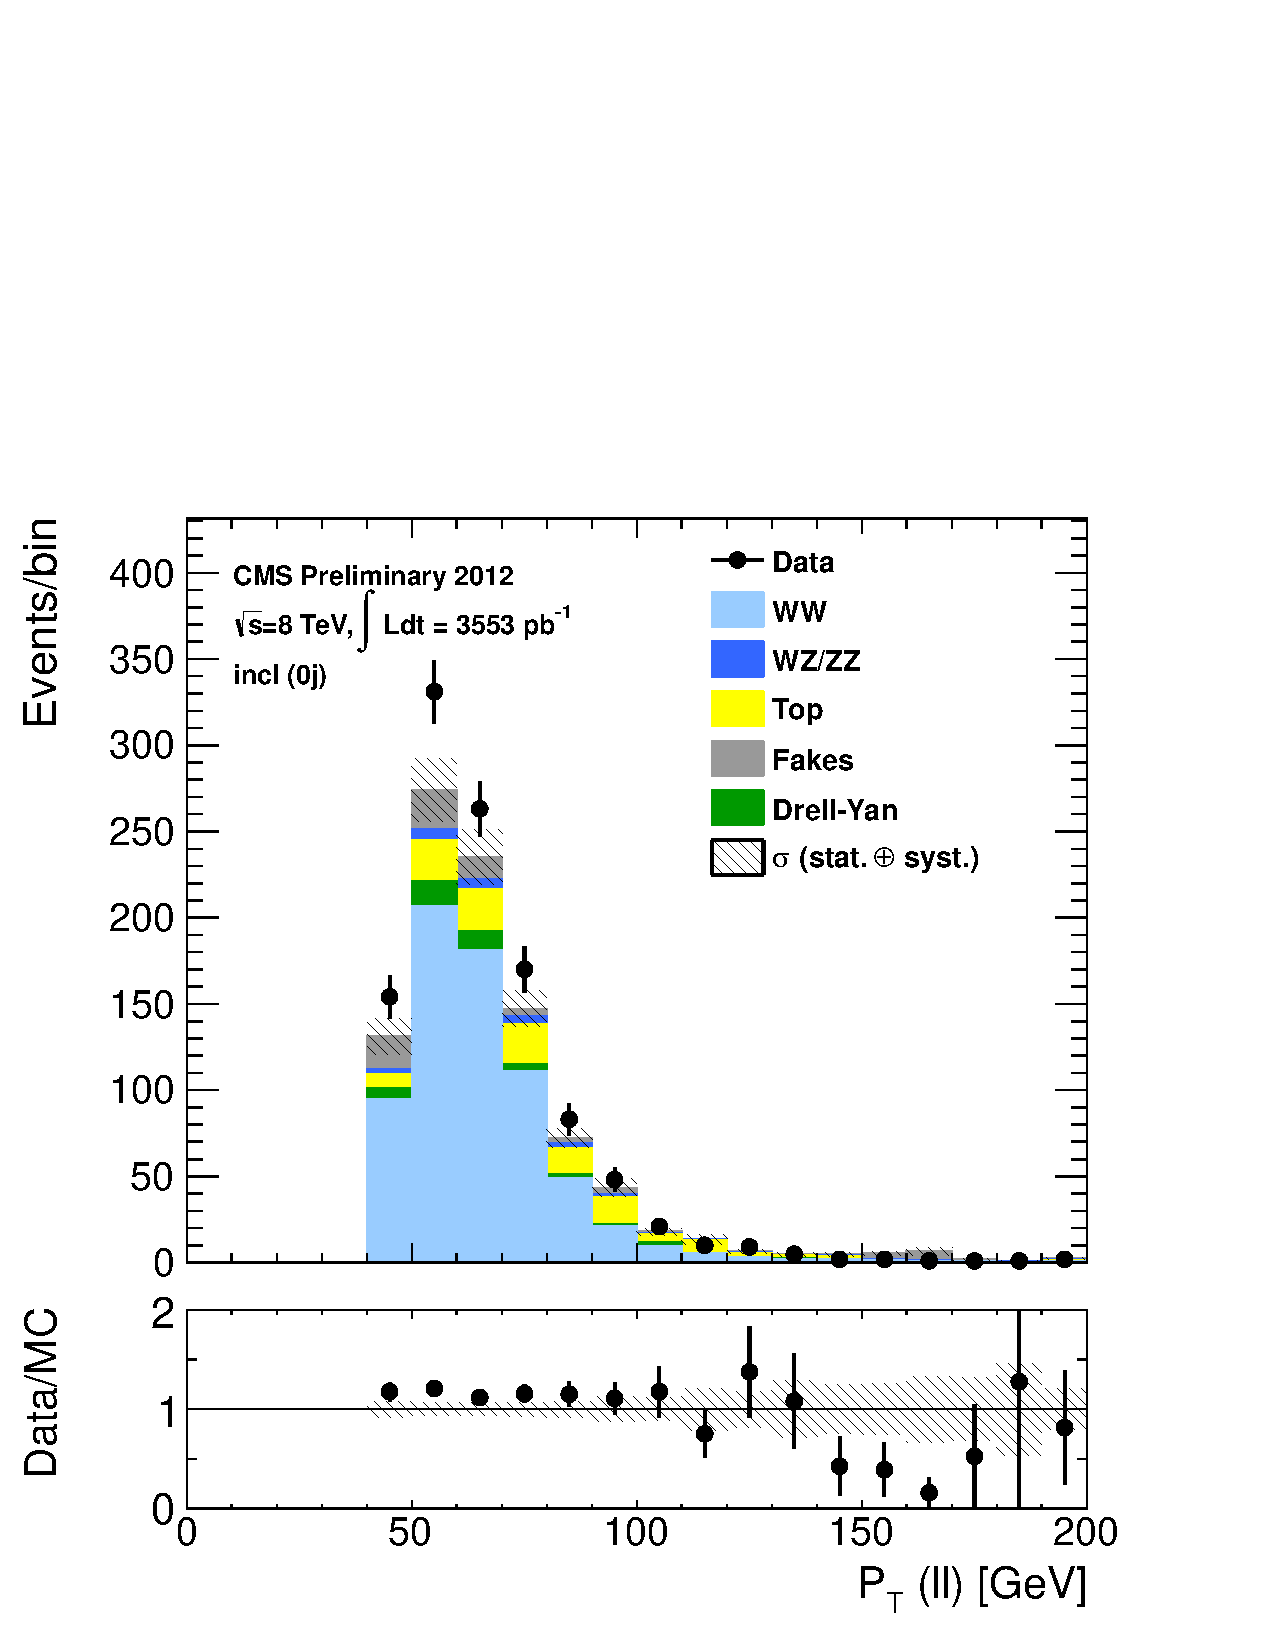
\includegraphics[width=.45\textwidth]{figures/ww_analysis20_ptll_incl_0j.pdf}}
\subfigure[Dilepton system invariant mass]{\label{subfig:fig_inclplots_M}
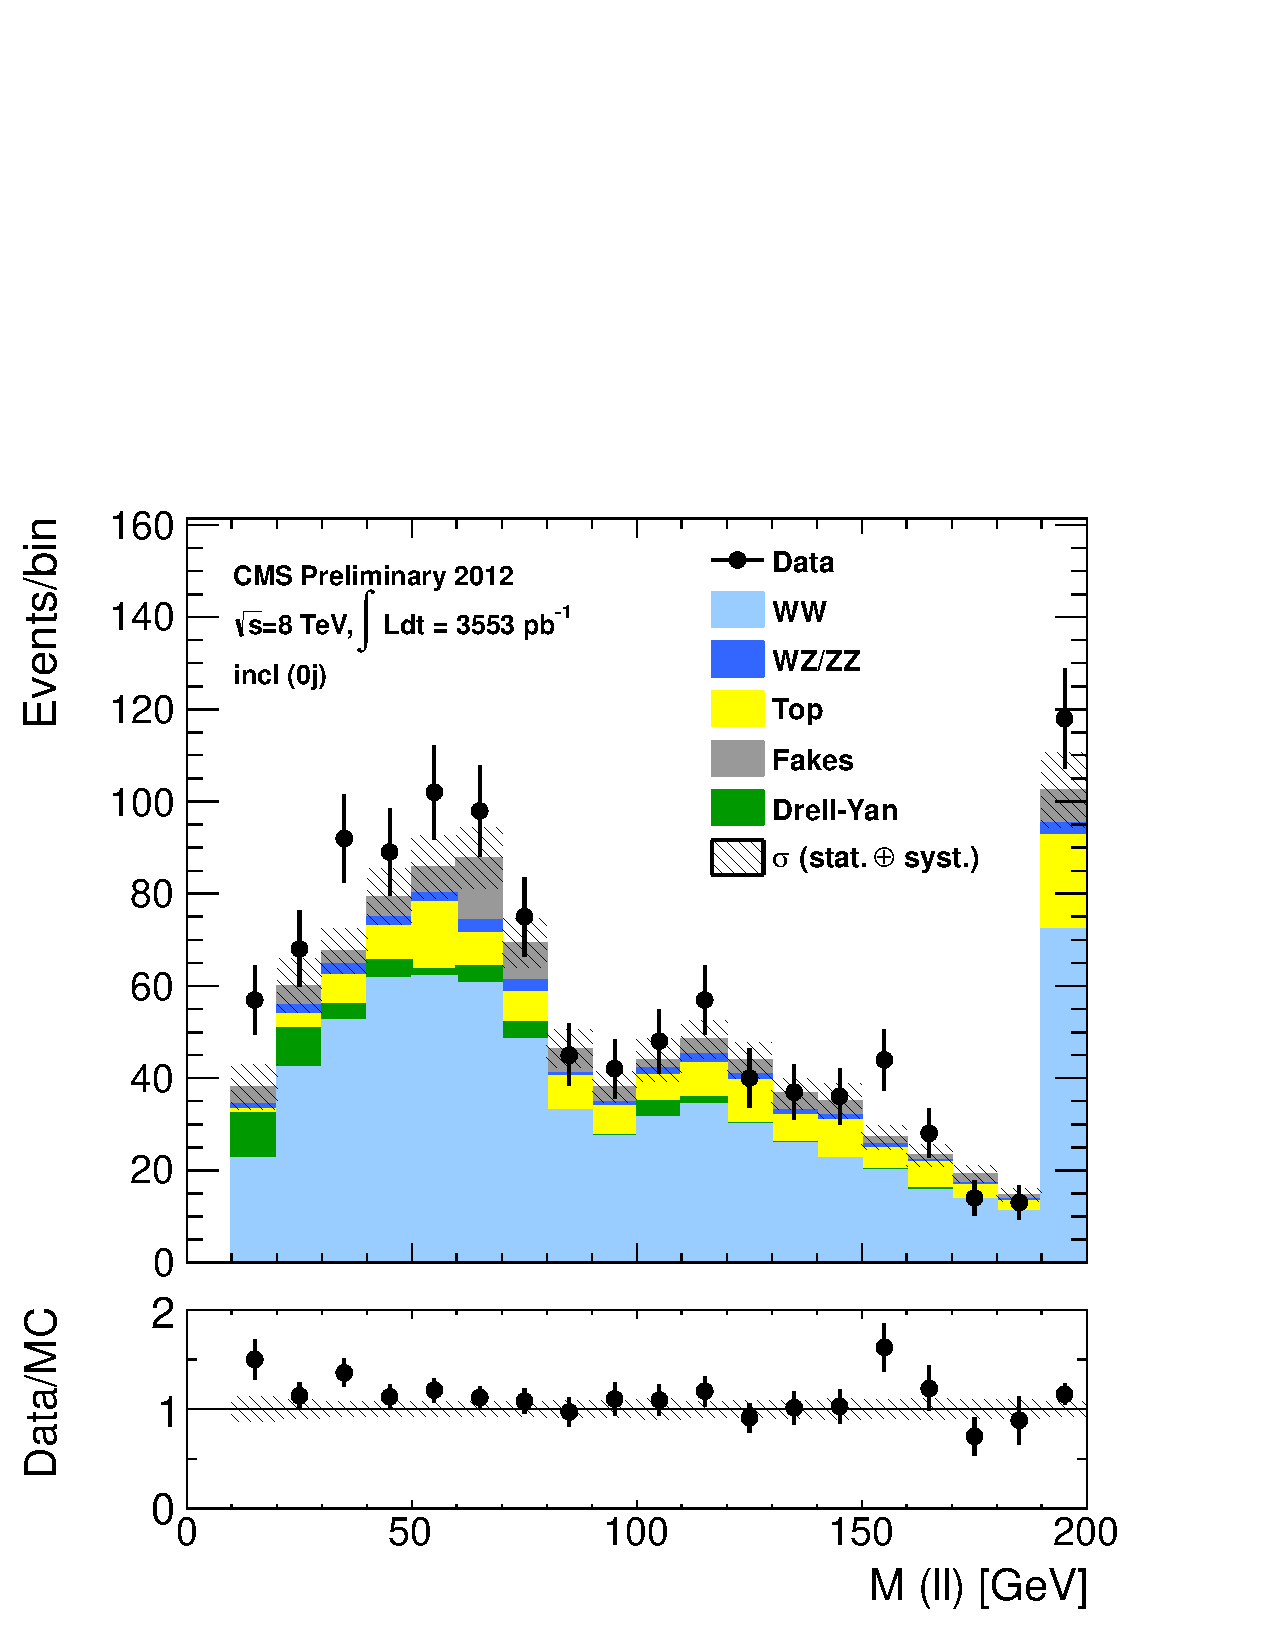
\includegraphics[width=.45\textwidth]{figures/ww_analysis20_mll_incl_0j.pdf}}
\caption{Kinematic distributions for expected and observed events in the  $\mu\mu$, $\mu{e}$, $e\mu$ and $ee$ channels.
%The dilepton system invariant mass distribution has the $Z$ mass veto relaxed.
The uncertainty on the expected events includes both statistical and systematic components.}
\label{fig:inclplots}
\end{center}
\end{figure}
%%%%%%%%




